\documentclass[hyperref, bachelorofscience]{cgvpub}
% other document types next to bachelorofscience:
% masterofscience
% diplominf
% diplomist
% beleg

%more options (to be appended in the square brackets):
% german....... german version 
% female........ to be used for female endings in german
% bibnum....... numerical reference style
% final............ intended for the final submission
% lof.............. genereate list of figures
% lot.............. generate list of tables
% noproblem.. do not show task
% notoc......... do not generate table of contents
% twoside...... two sided layout


\author{Lucas Waclawczyk}
\title{Development of a Natural VR User Interface Using Haptic Gloves}
\birthday{26. April 1998}
\placeofbirth{Bad Langensalza}
\matno{4686687}
\betreuer{Prof. Stefan Gumhold}
\bibfiles{lib.bib}
\problem{Write down your task...}
\copyrighterklaerung{\textbf{Voyager Bridge Mesh}\\
Acquired from \url{https://www.trekmeshes.ch/} on 20 June 2020.

This mesh remains the property of Chainsaw\_NL and Star trek Meshes.
It however may be used to create images and scenes for non-profit use only.

Any images produced with this mesh do NOT have to be credited to the
mesh author. But it would be nice.

Star Trek and Enterprise are copyright Paramount Pictures.}
\acknowledgments{I'd like to thank...}
\abstracten{abstract text english}
\abstractde{ abstract text german}

\usepackage{subcaption}
\usepackage{algpseudocode}

\usepackage{glossaries}
\newglossary[tlg]{gloss_terms}{tld}{tdn}{Glossary}
\newglossary[slg]{gloss_acr}{sot}{stn}{Acronyms}
\makeglossaries
\loadglsentries[gloss_terms]{gloss_terms}
\loadglsentries[gloss_acr]{gloss_acr}

\newcommand{\newcite}[1]{$ ^{\text{\cite{#1}}} $}

\begin{document}
\glsaddall
	
\chapter{Introduction}
What makes a good \acrfull{vr} application? What qualities should it have and how well developed is the necessary technology? In their review \emph{Haptic display for virtual reality: progress and challenges}\newcite{wang19}, Wang et al. state that \gls{vr} was born in 1965 with Ivan Sutherlands proposal of a concept named "The Ultimate Display"\newcite{sutherland65}. In that report of the IFIP Congress, Sutherland names immersion, interaction and imagination as three important features of \acrshort{vr}. 

There has been a multitude of approaches to making interaction with virtual environments possible\newcite{li19}. Touch screens and stylus pens have become quite common in everyday life. Devices capable of capturing scene depth like Microsoft Kinect and Leap Motion make touchless interaction possible, e.g. during games. This thesis focuses especially on wearable devices called \emph{data gloves}.

\section{Principles of Data Gloves}
The general principles of data gloves can be divided into two main parts: sensing and actuation. The first part deals with the issue of capturing a user's hand poses and motions and relaying that information to a computer for further processing. In most cases, a fabric glove is equipped with an \acrfull{imu} placed on each rigid hand part or flex sensors placed on joints. The latter have the advantage of measuring absolute values which, however, are only scalar and need further interpretation involving anatomical knowledge ("Something is happening: we have a $ .7 $."). An \acrfull{imu}, on the other hand, usually accumulates an absolute measurement from instantaneous rates of change, but can be designed to return 3D rotations and positions ("The index is facing upwards.").

The matter of actuation belongs to the broader field of haptic feedback. According to Wang et al.\newcite{wang19}, the visual and auditory feedback of \acrshort{vr} systems has become fairly realistic over time. However, haptic feedback is still rather poor even though it is "$\dots$ indespensable for enhancing immersion, interaction and imagination of \acrshort{vr} systems. Interaction can be enhanced by haptic feedback as users can directly manipulate virtual objects, and obtain immediate haptic feedback. Immersion of the \acrshort{vr} system can be enhanced in terms of providing more realistic sensation to mimic the physical interaction process. Imagination of users can be inspired when haptics can provide more cues for user[s] to mentally construct an imagined virtual world beyond spatial and or temporal limitations."

\begin{figure}
	\centering
	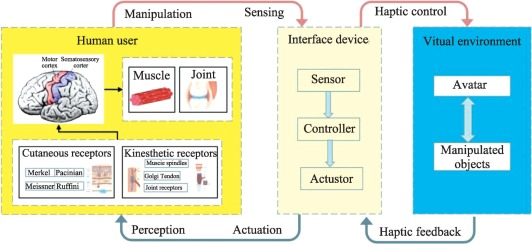
\includegraphics[width=.8\linewidth]{../pics/wang01}
	\caption[Schematic paradigm of haptic human computer interfaces]{Schematic paradigm of haptic human computer interfaces consisting of three components, i. e. human user, interface device, and virtual environment; from \cite{wang19}}
	\label{fig:hci}
\end{figure}

A schematic of the general paradigm of haptic human computer interfaces is shown in figure \ref{fig:hci}. It consists of three main components:
\begin{itemize}
	\item the user, who perceives virtual objects through biological receptors, processes them in the somatosensory and motor cortex, and requests manipulation by mechanical movement,
	\item the interface device which causes perception via actuation and collects information about requested manipulation with its sensors,
	\item the virtual environment which evaluates the interface device's data, realizes the manipulation of virtual objects with possible constraints, and motivates actuation in the interface device via haptic feedback.
\end{itemize}

As the following examples will demonstrate, not all data gloves are designed with the capability of both sensing and actuation. Some are only used to evaluate the user's hand pose, and it is conceivable to deal only with the issue of actuation and utilize an external device for sensing, such as Leap Motion. However, actuation on its own does not seem useful, as it needs to variable based on the current hand pose.

\section{Examples and Applications of Data Gloves}
\subsection{Sign Language Recognition}
In 2018, Kakoty et al. developed a data glove and processing system for the recognition of sign language alphabets (Indian, American and numbers) and their translation into speech\newcite{kakoty18}. In their paper, several earlier projects with similar purposes are reviewed, most of which are vision based. The authors point out that glove based systems are more useful because they "[$\dots$] allow one with the freedom for locomotion during the recognition process and [are] independent of the environmental lighting conditions."

\begin{figure}
	\begin{subfigure}{.4\linewidth}
		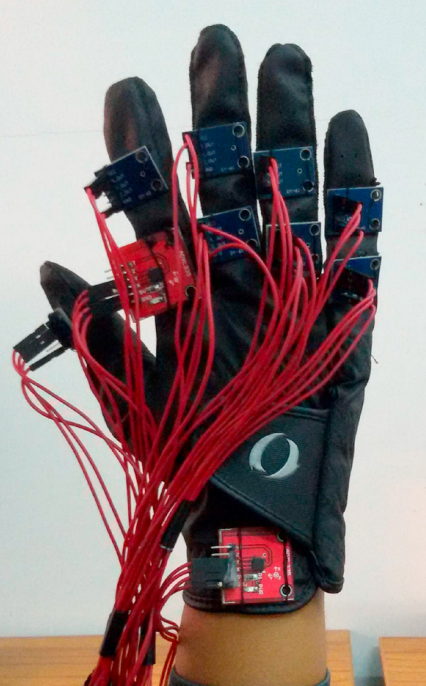
\includegraphics[width=\linewidth]{../pics/kakoty_glove}
		\caption{Data glove developed by Kakoty et al.}
		\label{fig:kakoty_glove}
	\end{subfigure}
	\hfill
	\begin{subfigure}{.43\linewidth}
		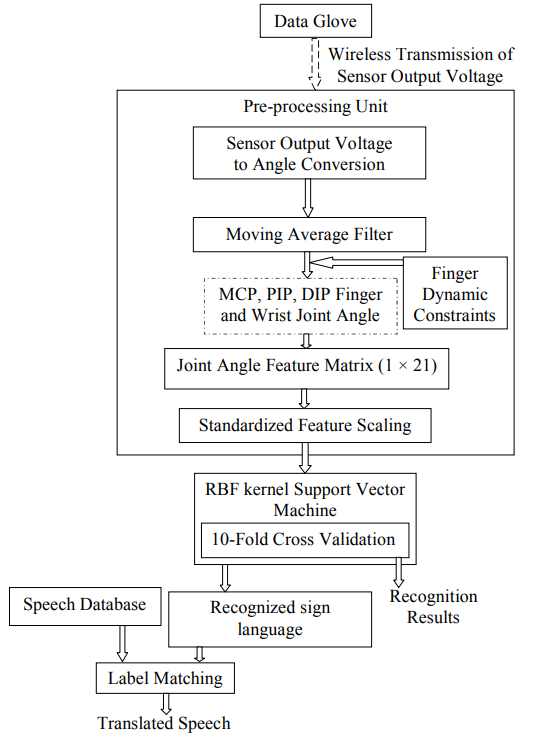
\includegraphics[width=\linewidth]{../pics/kakoty_principle}
		\caption{Proposed methodology for sign language recognition}
		\label{fig:kakoty_principle}
	\end{subfigure}
	\caption[A system for sign language recognition]{A system for sign language recognition; from \cite{kakoty18}}
	\label{fig:kakoty}
\end{figure}

The data glove used for this project is shown in figure \ref{fig:kakoty_glove}. It was constructed from a leather glove by equipping it with ten angle sensors, a microcontroller, and a transceiver module. The original paper describes this design in detail.

A preprocessing unit as in figure \ref{fig:kakoty_principle} handles the conversion from sensor output voltage to denoised, constrained standardized feature vectors. These are then processed by a radial base function kernel support vector machine and finally, the recognized sign language is translated into speech using label matching with a pre-recorded speech database. The whole process is implemented to run in real-time with the sensor data acquisition.

With an average recognition rate of 96.7\%, this approach achieves similar results as previous projects while recognizing more alphabets. Kakoty et al. further conclude that their approach "[$\dots$] overcomes the limitations of vision based systems. [$\dots$] An extension of the presented work for sentence-based sign language recognition will lead to an enterprising device; which is part of on-going research."

\subsection{Daily Activity Recognition}
Alzheimer's disease is a common cause for the loss of cognitive abilities amongst the elderly. Well known symptoms include language problems, loss of memory and degrading functioning of the hand. To better understand the latter, Maitre et al. investigated a method to recognize daily activities using a data glove developed over the course of the project\newcite{maitre19}.

\begin{figure}
	\begin{subfigure}{.57\linewidth}
		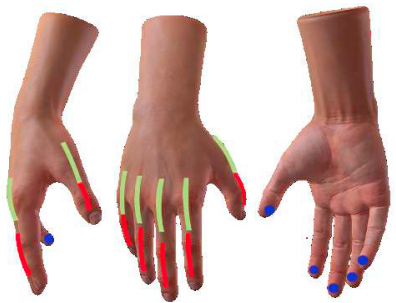
\includegraphics[width=\linewidth]{../pics/maitre_sensors}
		\caption{Arrangement of sensors on the hand}
		\label{fig:maitre_sensors}
	\end{subfigure}
	\hfill
	\begin{subfigure}{.3\linewidth}
		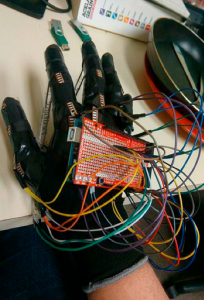
\includegraphics[width=\linewidth]{../pics/maitre_glove}
		\caption{Prototype device}
		\label{fig:maitre_glove}
	\end{subfigure}

	\vspace{.5cm}
	\begin{subfigure}{\linewidth}
		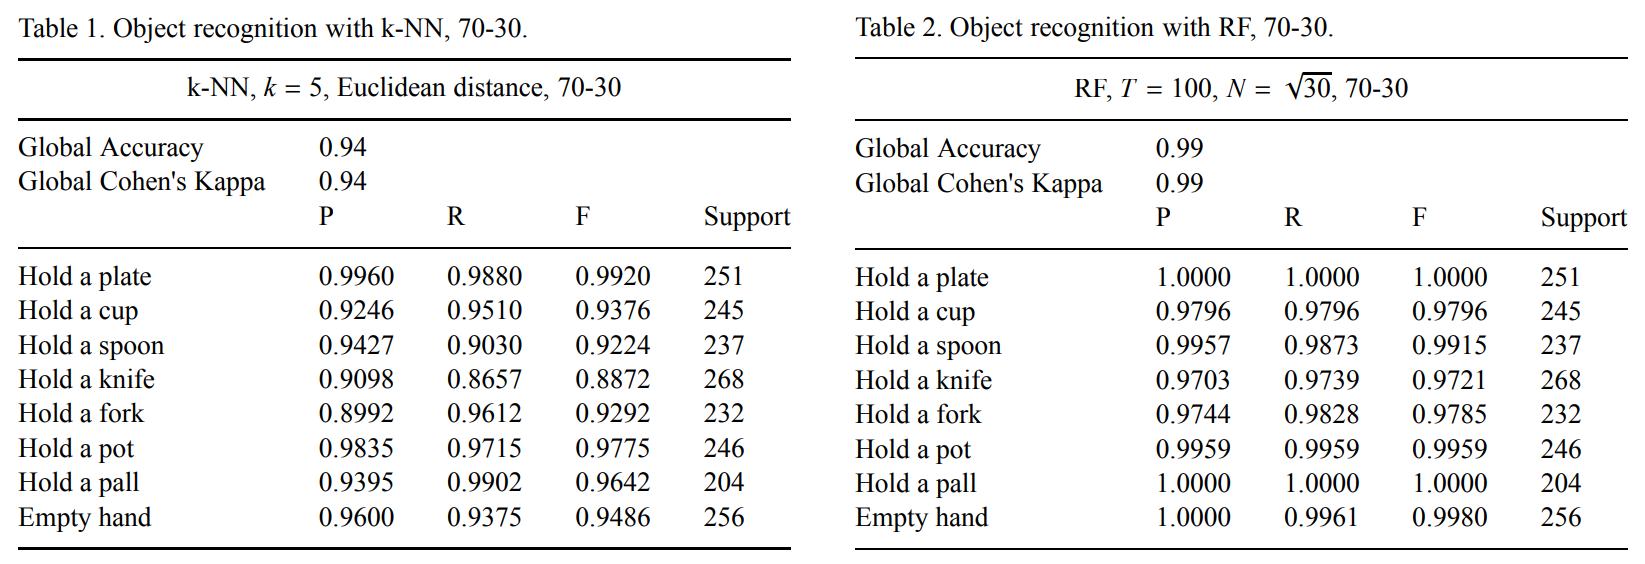
\includegraphics[width=\linewidth]{../pics/maitre_results}
		\caption{Evaluation of the recognition results}
		\label{fig:maitre_results}
	\end{subfigure}
	\caption[A data glove for recognition of basic daily activities]{A data glove for recognition of basic daily activities; from \cite{maitre19}}
	\label{fig:maitre}
\end{figure}

Several reasons are named as motivation to develop the device from scratch:
\begin{itemize}
	\item Prices for commercial data gloves are situated between ca. 600 USD and several thousand USD. The authors propose a design that can be recreated for only about 220 USD.
	\item Commercial gloves are generally only compatible with Windows, but the SDK is not suitable for many other sensors.
	\item The new design can be specialized for recognizing the required types of grasp.
\end{itemize}

Discerning a daily activity is based on recognizing the involved item, e.g. a plate for the task \emph{Hold a plate}. For this, the presence of an object needs to be detected and information about its shape is required. Figure \ref{fig:maitre_sensors} shows the resulting sensor locations, where red and yellow mark flex sensors and blue marks force sensors. A prototype device can be seen in figure \ref{fig:maitre_glove}. 

A group of nine participants was asked to perform the daily activities listed in the evaluation tables in figure \ref{fig:maitre_results}. The acquired data sets were used to train (70\%) and test (30\%) a k Nearest Neighbours (k-NN) model whose precision (P), recall (R) and f-score (F) can be found in the left table, and a random forest (RF) to which the right table refers.

Maitre et al. conclude that the performance of their approach is "[$\dots$] almost perfect [$\dots$]. This result is surprising and encouraging [$\dots$]." Another experiment shows that both models perform significantly worse on data collected from a person that was not recorded during training. The authors therefore suggest to train the models with data from a patient that is supposed to use the system. The device can then even be worn in the comfort of the patient's home to monitor their hand activity.

\subsection{Refined Myoelectric Control in Below-Elbow Amputees}
\begin{figure}
	\centering
	\begin{subfigure}{.35\linewidth}
		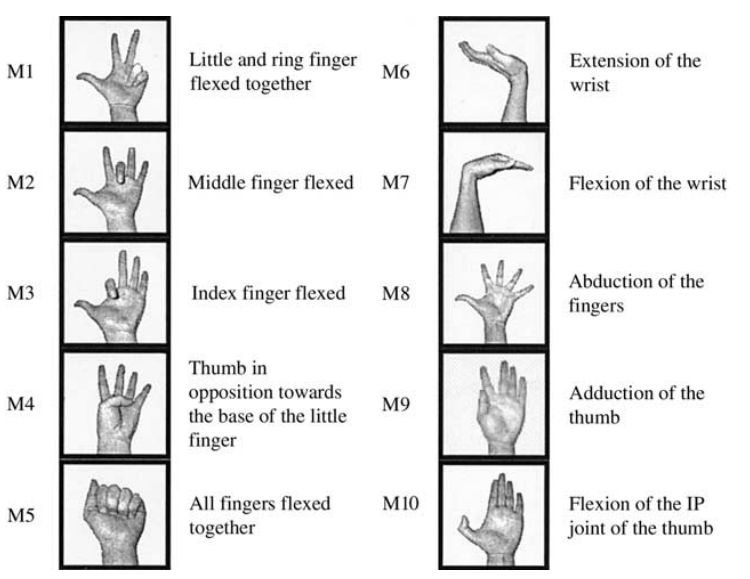
\includegraphics[width=\linewidth]{../pics/amputees_poses}
		\caption{Hand poses performed during training data acquisition}
		\label{fig:amputees:poses}
	\end{subfigure}
	\hfill
	\begin{subfigure}{.3\linewidth}
		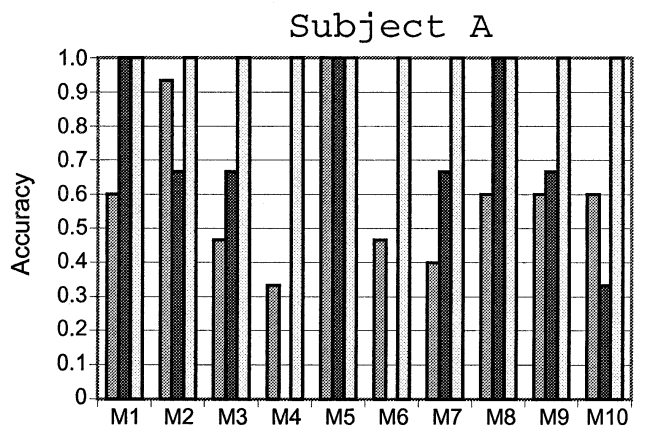
\includegraphics[width=\linewidth]{../pics/amputees_a}
		\caption{Recognition results of phantom hand movements for a subject with traumatic amputation (Subject A)}
		\label{fig:amputees:a}
	\end{subfigure}
	\hfill
	\begin{subfigure}{.3\linewidth}
		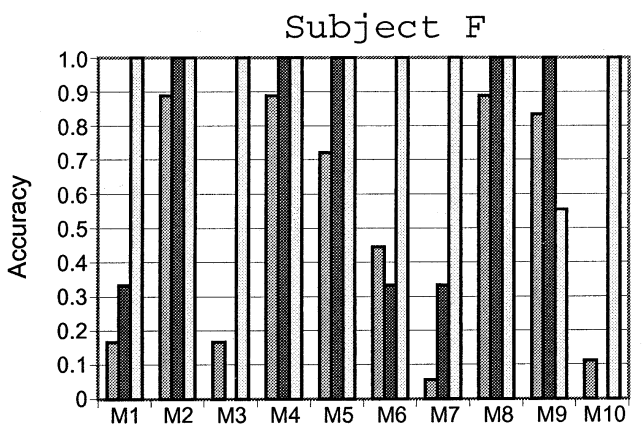
\includegraphics[width=\linewidth]{../pics/amputees_f}
		\caption{Recognition results of phantom hand movements for a subject with congenital failure of formation (Subject F)}
		\label{fig:amputees:f}
	\end{subfigure}
	\caption[Hand poses used in \cite{sebelius05} and recognition results]{Hand poses used in \cite{sebelius05} and recognition results; in (b) and (c), grey bars depict average performance, black depicts best-session performance and white the reference glove performance}
	\label{fig:amputees}
\end{figure}

A group of PhD students in Sweden trained an \acrfull{ann} to recognize myoelectric activity of below-elbow amputees as certain hand poses\newcite{sebelius05}. To generate training data, a group of five subjects with a traumatic amputation and one subject with a congenital failure of formation was asked to perform the movements shown in figure \ref{fig:amputees:poses} with their healthy hand and their phantom hand simultaneously.

The healthy hand was therewhile tracked with a data glove to match the performed movement to one of M1 - M10. The arm stump on the side of the amputation was covered with considerably many electrodes to record detailed information about the remaining myoelectric activity. The (pre-processed) data was then used to train a tree-structured \acrshort{ann}.

As shown in figure \ref{fig:amputees} and more diagrams from the original paper, certain poses were recognized especially well or badly for certain subjects. An interesting process to see was how the performance of the subjects became more accurate over the course of the experiment. As this could be seen within minutes, the authors theorized, it might be due to unmasking of existing brain structures instead of the formation of new ones. 

The subject with congenital failure was of special interest because it showed that some movements could be accurately induced in the phantom hand even though they had never been executed before, possibly indicating the awakening of sleeping motor cortical areas in the brain that had been present since birth. Among the subjects with traumatic amputations, the accuracy and training effect did not seem related to the time since the amputation.

An important aspect for the training effect might be the simultaneous execution of movements with the healthy hand, as suggested in the original paper. The authors moreover suppose that a subject's performance might increase with visual feedback of a virtual phantom hand that was not present during these experiments. This thesis might be useful for this purpose, as it describes the use of a well established hand model in section \ref{sec:hand_model}. Work in this direction was continued by the authors of the original paper\newcite{sebelius06}.

\subsection{Commercial Products}
Dexmo, CyberGrasp, \Gls{AVR}

\subsection{A Lightweight Force-Feedback Glove}

\chapter{Development}
\section{Devices and Software}
\begin{figure}
	\begin{subfigure}{.49\linewidth}
		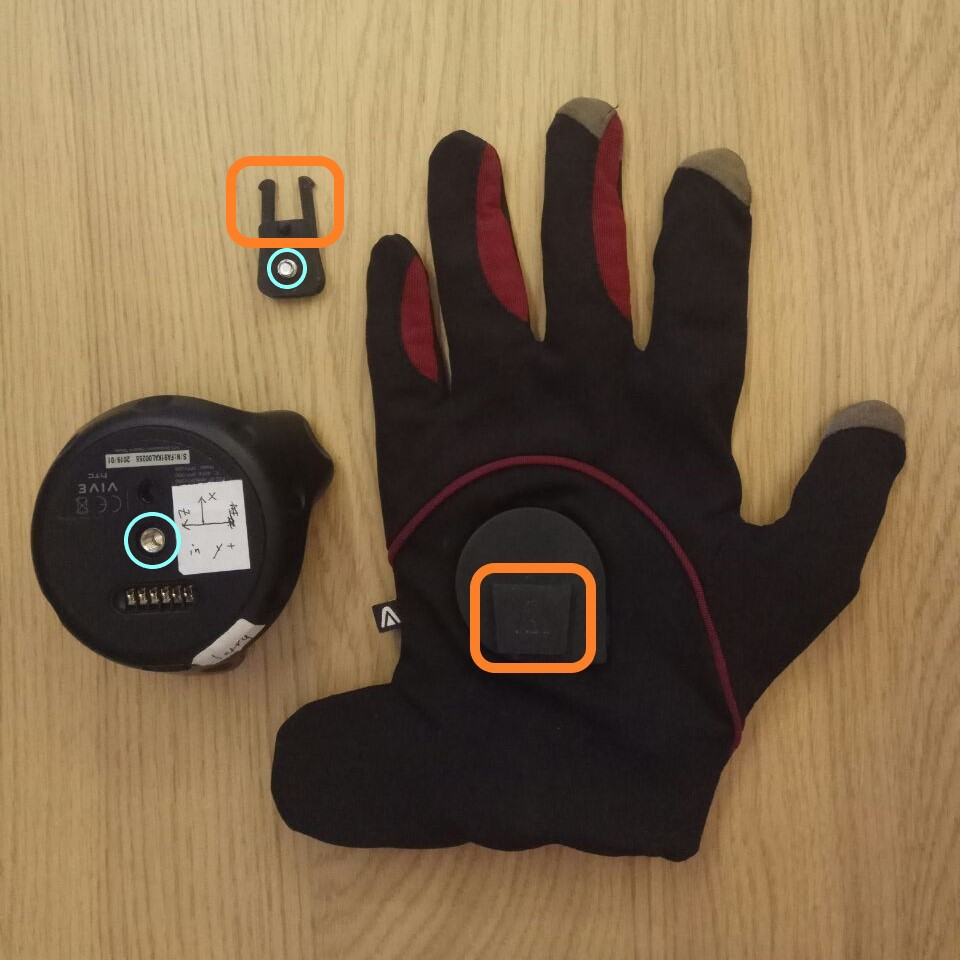
\includegraphics[width=\linewidth]{../pics/devices_uncoupled}
		\caption{Uncoupled devices, colors mark coupling points}
		\label{fig:devices:unc}
	\end{subfigure}
	\hfill
	\begin{subfigure}{.49\linewidth}
		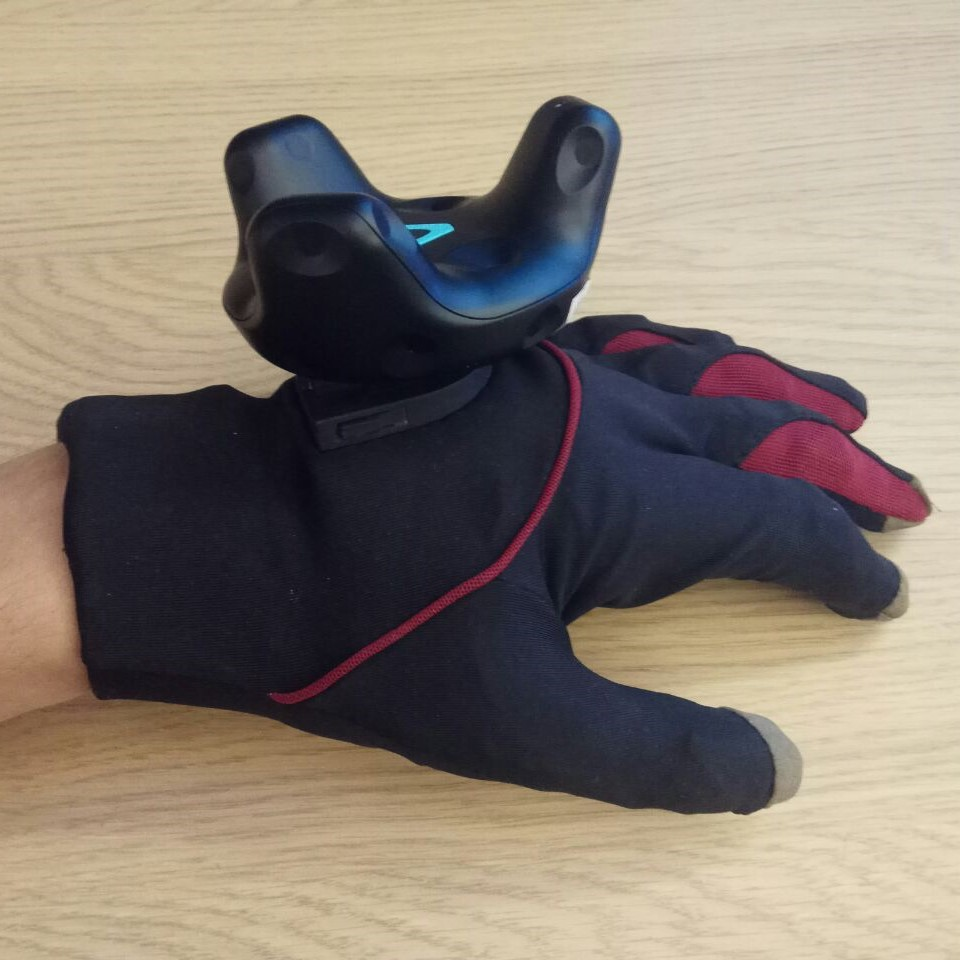
\includegraphics[width=\linewidth]{../pics/devices_coupled}
		\caption{Coupled devices on user hand}
		\label{fig:devices:cou}
	\end{subfigure}
	\caption[Devices used to track the user's hand]{Devices used to track the user's hand: Vive tracker, coupling, Avatar VR}
	\label{fig:devices}
\end{figure}

For the purpose of thesis, I used a pair of haptic gloves called Avatar VR which is a registered trademark of NeuroDigital Technologies, S. L.\newcite{nd}, referred to as \acrshort{nd} hereafter..

To use the Avatar VR on a computer, one needs to download, install and run the \acrshort{nd} Suite. This program provides a background service and GUI for managing and accessing the devices. A connection can be established via Bluetooth after which all sensor data is graphically displayed in the GUI.

\acrshort{nd} also supplies a developer's API in the form of three files (\lstinline|NDAPI.h, NDAPI_x64.lib and NDAPI_x64.dll| or \lstinline|x86| respectively) which need to be included into the respective project in a suitable manner. An instance of the \lstinline|NDAPI.h| can be used to access the data of devices connected to \acrshort{nd} Suite.

Additionally, a Vive tracker was used to determine the user's hand position and orientation. The Avatar VR can be mechanically connected to the tracker using a coupling, that needs to be acquired separately. The devices named so far and the way of coupling them can be seen in figure \ref{fig:devices}.

The foundation for the graphics software I developed is implemented in the \gls{CGV} framework provided by the chair of computer graphics and visualization at TU Dresden.

A user can view the plugin on a computer screen with the \lstinline|cgv_viewer| or on a \Gls{VIVE} \acrfull{hmd} simply by connecting one to the computer.

\section{Project Idea and Structure}
\begin{figure}
	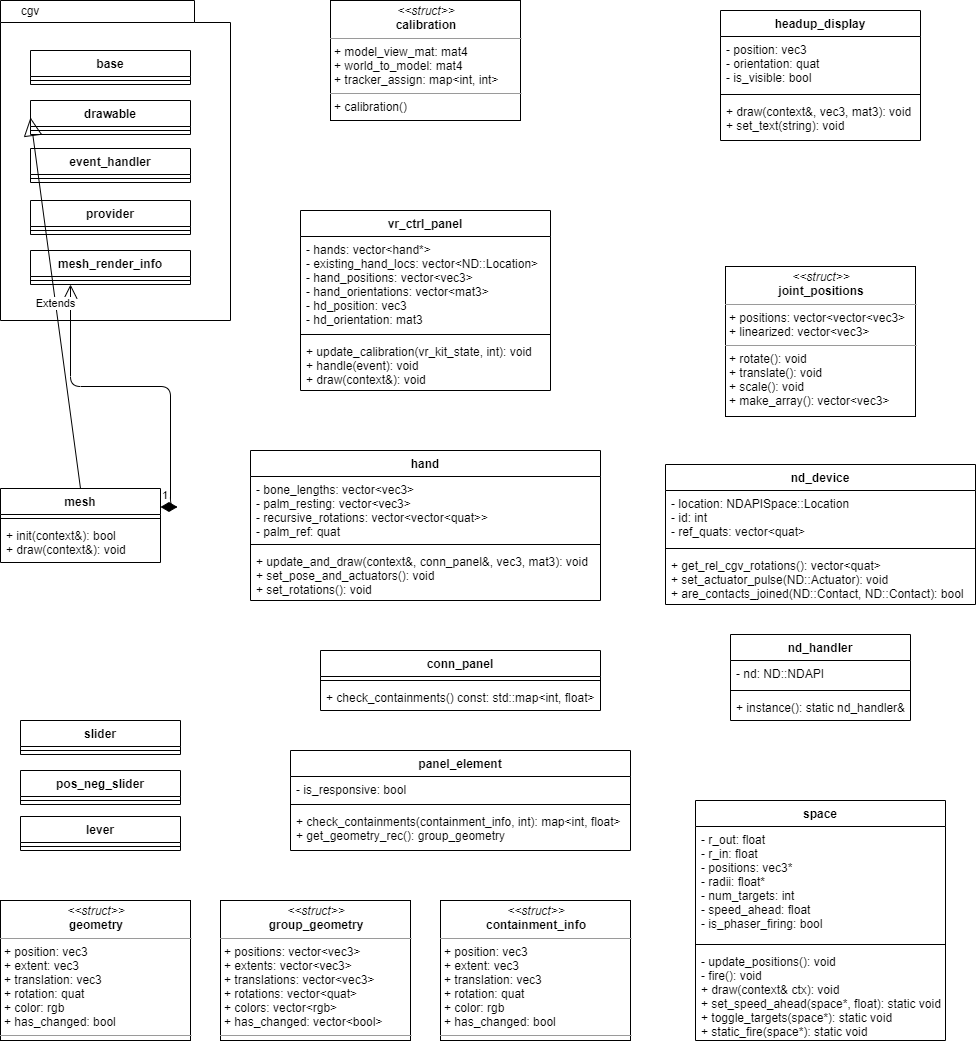
\includegraphics[width=\linewidth]{../pics/uml}
	\caption[Class diagram of \gls{VCP}]{Class diagram of \gls{VCP}, only most relevant elements shown}
	\label{fig:uml}
\end{figure}

The following sections describe the development of a VR user interface utilizing these technologies in real-time. To give this some context rather than just moving boxes, I decided to design it as a conn panel on the USS Voyager (Star Trek). The term \emph{conn} is short for \emph{control and navigation}, meaning the panel is used to stear the ship. The classes used to implement this and their interaction are shown in figure \ref{fig:uml}.

The main class and entry point carries the same name as the plugin itself. It is derived from the \gls{CGV} classes \lstinline|base|, \lstinline|drawable|, \lstinline|event_handler| and \lstinline|provider|, and used for management of all objects. Its capability to handle \lstinline|vr_pose_events| is used to forward tracker poses (position and orientation) to the \lstinline|hands| and \acrshort{hmd} poses to the \lstinline|head_up_display|. It distributes \lstinline|draw()| commands among the relevant members and manages the calibration routine described in section \ref{sec:cal}. This is the only class registered via object registration.

Written information can be displayed to the user with the \lstinline|head_up_display| if an \acrshort{hmd} is connected and on the console alternatively. The \lstinline|head_up_display| is permanently adjusted to be displayed in the upper left corner of the user's visual field.

The \lstinline|mesh| class renders the Voyager bridge. It uses the basic functionality of \lstinline|mesh_render_info| provided in \gls{CGV} to load and draw.

Around the bridge, space is simulated by a spherical shell filled with stars. The user never actually changes position in model space. Instead, stars are moved in the opposite direction of the simulated motion, the speed of which can be set via static \lstinline|set_speed_*()| methods. The details of this are described in section \ref{sec:space}.

All interactive elements are implemented as \lstinline|panel_node| or its derived classes. A \lstinline|conn_panel| constructs and manages a tree of such nodes. Elements are represented as boxes and combinations of boxes placed relative to their parent element. The \lstinline|slider| and \lstinline|lever| classes require a callback function and pointer to a \lstinline|stars_sphere| as arguments in their constructor that are used to set some speed in the \lstinline|stars_sphere|. The \lstinline|conn_panel| is positioned right on top of the mesh's conn.

Interaction with the \Gls{AVR} is managed by the singleton \lstinline|nd_handler| which can be used to pass function calls through to an instance of \lstinline|NDAPI|. This is frequently done in \lstinline|nd_device|, a class for querying sensor data from the gloves and converting it for better compatibility with \lstinline|cgv| and \gls{VCP}.

Finally, a representation of the user's hands is implemented in \lstinline|hand|. It keeps track of several points and joints the details of which are described in section \ref{sec:hand_model}. During a \lstinline|draw()| call, \lstinline|vr_ctrl_panel| passes a pointer to its \lstinline|conn_panel| to each \lstinline|hand| which then passes on information about the current hand geometry wrapped as \lstinline|containment_info| to the \lstinline|conn_panel| for containment check. During this check, each \lstinline|panel_node| containing some hand part can react with its \lstinline|on_touch()| method. A \lstinline|map<int, float>| describing the contained positions is returned to the hand, enabling it to react as well.

\section{Skeletal Hand Model for the Avatar VR Haptic Glove} \label{sec:hand_model}
\subsection{Abstraction of the Human Hand Skeleton}
\begin{figure}
	\begin{subfigure}{.5\linewidth}
		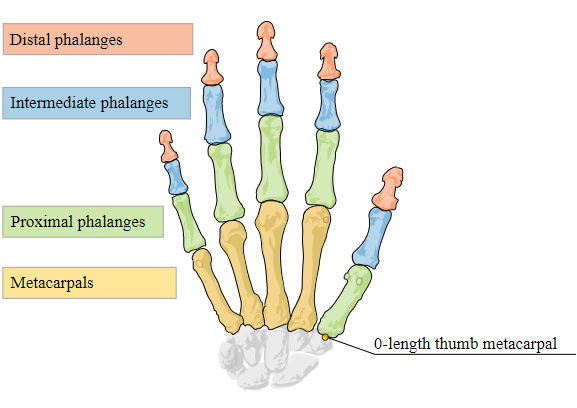
\includegraphics[width=\linewidth]{../pics/leap_anat}
		\caption{General bone structure of the human hand}
		\label{fig:hand_model:anat}
	\end{subfigure}
	\hfill
	\begin{subfigure}{.47\linewidth}
		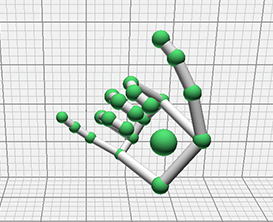
\includegraphics[width=\linewidth]{../pics/leap_example}
		\caption{Screenshot of an example hand representation in the Leap Motion API version 2.0, cropped}
		\label{fig:hand_model:leap}
	\end{subfigure}
	\caption{A model of the human hand; from \cite{leaphand}}
	\label{fig:hand_model}
\end{figure}

The human hand can be roughly divided into the parts shown in figure \ref{fig:hand_model:anat}, i.e. the \emph{\glspl{MC}}, \emph{\glspl{PPh}}, \emph{\glspl{IPh}}, and \emph{\glspl{DPh}}. A joint connecting a \gls{MC} to a \gls{PPh} is called \emph{\gls{MPJ}}, and followed by a \emph{\gls{PIJ}} and a \emph{\gls{DIJ}}.

Even though the carpals (grey in figure \ref{fig:hand_model:anat}) are physiologically quite relevant for hand movement, they stay relatively fixed compared to the other bone sets, and can thus be omitted in our simplified model. In anataomical nomenclature, the thumb is composed of \gls{PPh} and \gls{DPh} only and follows a \gls{MC}. However, this model assumes a missing \gls{MC} and existing \gls{IPh} instead which will be modelled by a 0-length \gls{MC} for uniformity reasons.

The Leap Motion API version 2.0\newcite{leaphand} uses the abstraction described above and adds
\begin{itemize}
	\item an "end" joint per finger (at the end of the \gls{DPh})
	\item a joint diagonally across the palm from the \gls{MPJ} of the index
	\item a joint in the middle of the palm
\end{itemize}

The most common representation includes cylinders for the bones and spheres for the joints. It is shown in figure \ref{fig:hand_model:leap}.

\subsection{Technology and Function of the Avatar VR}
\begin{figure}
	\centering
	\begin{subfigure}{\linewidth}
		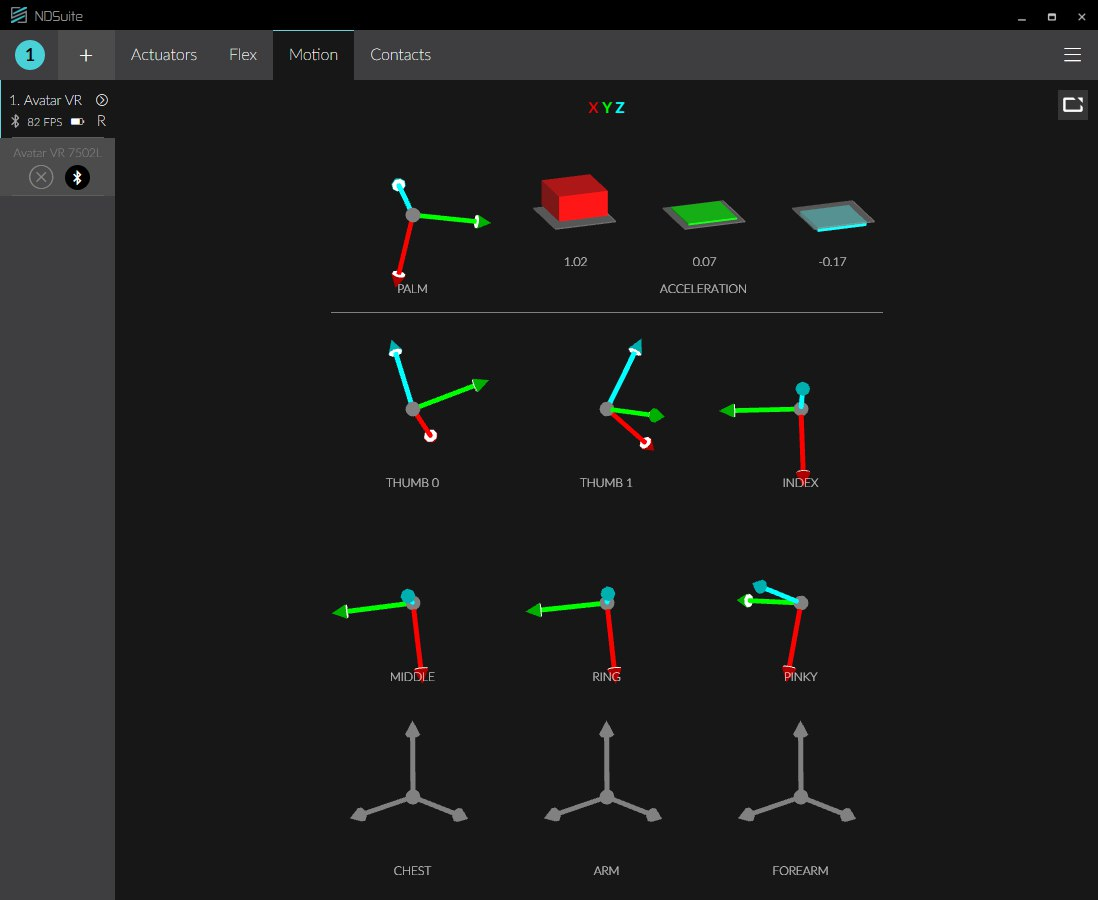
\includegraphics[width=\linewidth]{../pics/av_imus}
		\caption{"Motion" tab of ND Suite with orientations in an (optimistic) example hand pose}
		\label{fig:av_tech:imus}
	\end{subfigure}
	
	\vspace{.2cm}
	\begin{subfigure}{.45\linewidth}
		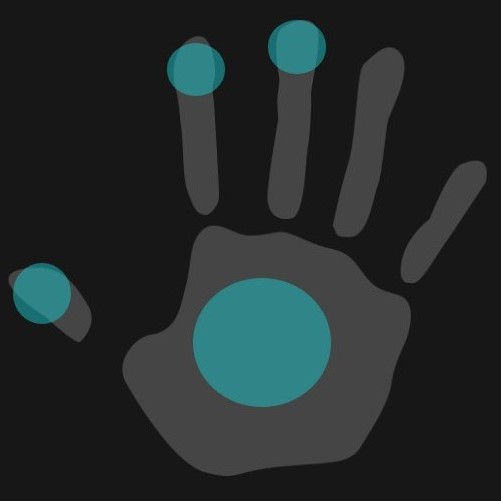
\includegraphics[width=\linewidth]{../pics/av_contacts}
		\caption{Positions of contact sensors}
		\label{fig:av_tech:contacts}
	\end{subfigure}
	\hspace{.3cm}
	\begin{subfigure}{.45\linewidth}
		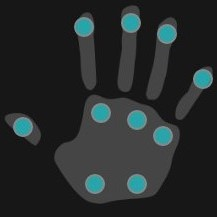
\includegraphics[width=\linewidth]{../pics/av_actu}
		\caption{Positions of actuators}
		\label{fig:av_tech:actuators}
	\end{subfigure}
	\caption{Sensors and actuators of the Avatar VR;\\screenshots of \acrshort{nd} Suite (b and c cropped)}
\end{figure}

The Avatar VR is equipped with three kinds of sensors: 
\begin{itemize}
	\item An \emph{\acrfull{imu}} is located on the \gls{IPh} of each finger to measure its 3D rotation. The thumb is even equipped with two \acrshort{imu}s (one per phalanx) and the palm with an \acrshort{imu} that can measure both 3D orientation and 3D rotation. The "Motion" tab of \acrshort{nd} Suite shown in figure \ref{fig:av_tech:imus} depicts the resulting orientations as orthonormal bases. 
	\item At the locations marked in blue in figure \ref{fig:av_tech:contacts}, the fabric is made of an electrically conductive material. These parts are used as contact sensors (short: contacts) to determine which of the marked locations are joined.
	\item The thumb also has a flex sensor, that will not be relevant for this thesis.
\end{itemize}

Furthermore, there are actuators at the locations marked in blue in figure \ref{fig:av_tech:actuators}. These can be used to generate vibrations of variable intensity as haptic feedback in a way that "[$\dots$] the brain perceives it as 'Real Touch' input", according to the producer.

\subsection{Using Data From the Avatar VR to Visualize the User's Hand}
The same model used by the Leap Motion API version 2.0 will also be used here. Leap captures absolute joint positions and optimizes them for visualization. In contrast, my approach for the Avatar VR is to use a fixed resting state geometry of the user's hand (bone lengths and resting state joint positions). At the time of a \lstinline|draw()| command, the geometry is adjusted according to the data given by the glove and the Vive tracker. The joint position data is managed by the struct shown in figure \ref{fig:joint_positions} (only most important parts included).

\begin{figure}
	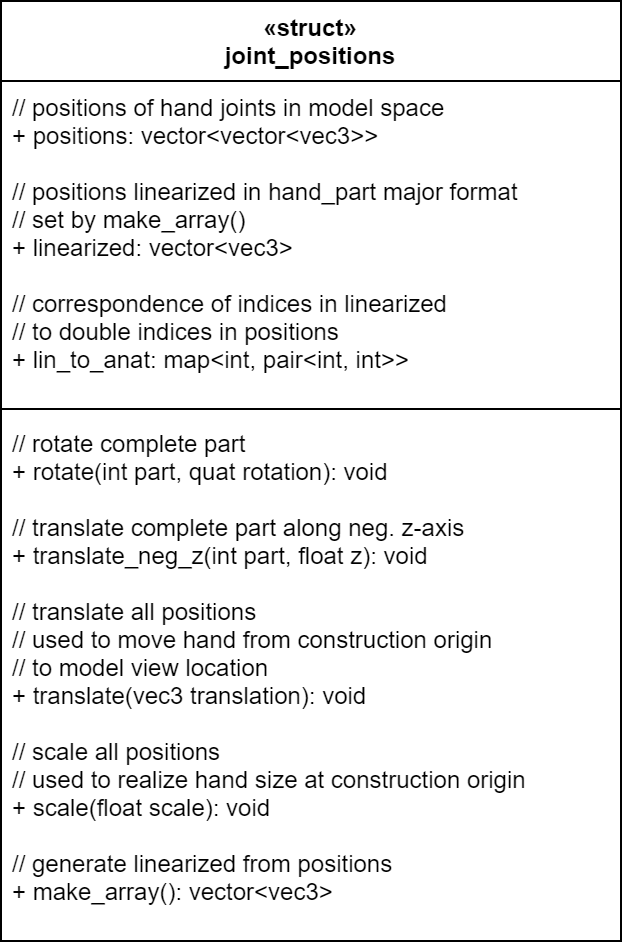
\includegraphics[width=.4\linewidth]{../pics/joint_positions}
	\caption{Struct for managing positions of hand joints}
	\label{fig:joint_positions}
\end{figure}

First, the palm joints' resting positions are rotated according to the orientation given by the Vive tracker. The construction of each finger begins at the end joint of the \gls{DPh} which is translated along the negative $ z $-axis by the hard-coded length of the \gls{DPh} and rotated by the respective quaternion (see below). The other phalanges are constructed in the same manner, before the whole finger is translated to the respective \gls{MPJ}. Finally, the whole hand is scaled to model view space and translated to the model view position of the Vive tracker.

Because the Avatar VR only returns one quaternion per finger (except for the thumb), I had to think of a way to distribute the orientation along all three phalanges: First, the Euler angles are calculated from the quaternion\newcite{quat_to_euler}
\begin{align*}
	\alpha \quad&=\quad \mbox{arctan} \frac {2(q_0 q_1 + q_2 q_3)} {1 - 2(q_1^2 + q_2^2)} \\
	\beta \quad&=\quad \mbox{arcsin} (2(q_0 q_2 - q_3 q_1)) \\
	\gamma \quad&=\quad \mbox{arctan} \frac {2(q_0 q_3 + q_1 q_2)} {1 - 2(q_2^2 + q_3^2)}
\end{align*}
where $ \alpha $ is the roll angle, $ \beta $ the pitch angle and $ \gamma $ the yaw angle, and the quaternion can be written as $ (q_{0}, q_{1}, q_{2}, q_{3}) $. For implementation, one has to use the \lstinline|atan2| function, because \lstinline|arctan| only return values between $ -\frac{\pi}{2} $ and $ \frac{\pi}{2} $.

The \lstinline|NDAPI| quaternions live in a space where the resting hand lies on the $ xz $-plane and the fingers point along the positive $ z $-axis. However, \gls{VCP} is oriented with the negative $ z $-axis as "front" direction, so $ q_{1} $ and $ q_{2} $ need to be negated before use. Then roll corresponds to bending the finger, pitch to a left-right-motion and yaw to a motion humans can hardly perform with their fingers.

Since the interphalangeal jionts act as revolute joints, only a roll component can be applied to them. As shown in the code below, the roll angle is distributed according to three floats (\lstinline|rot_split|). After some experimenting, $ (.5, .5, .25) $ is an option for these numbers that gives a good approximation of most actual hand poses. It corresponds to phalanx rotation during grabbing. Yaw and pitch are completely executed in the \gls{MPJ}. 
\begin{lstlisting}
	vec3 x(1, 0, 0), y(0, 1, 0), z(0, 0, 1);
	recursive_rotations[finger][PROXIMAL] = palm_rotation
		* quat(z, yaw) * quat(y, pitch) * quat(x, rot_split.x() * roll);
	recursive_rotations[finger][INTERMED] = quat(x, rot_split.y() * roll);
	recursive_rotations[finger][DISTAL] = quat(x, min(1.4f, rot_split.z() * roll));
\end{lstlisting}

\section{Simulation of Space} \label{sec:space}
\begin{figure}
	\centering
	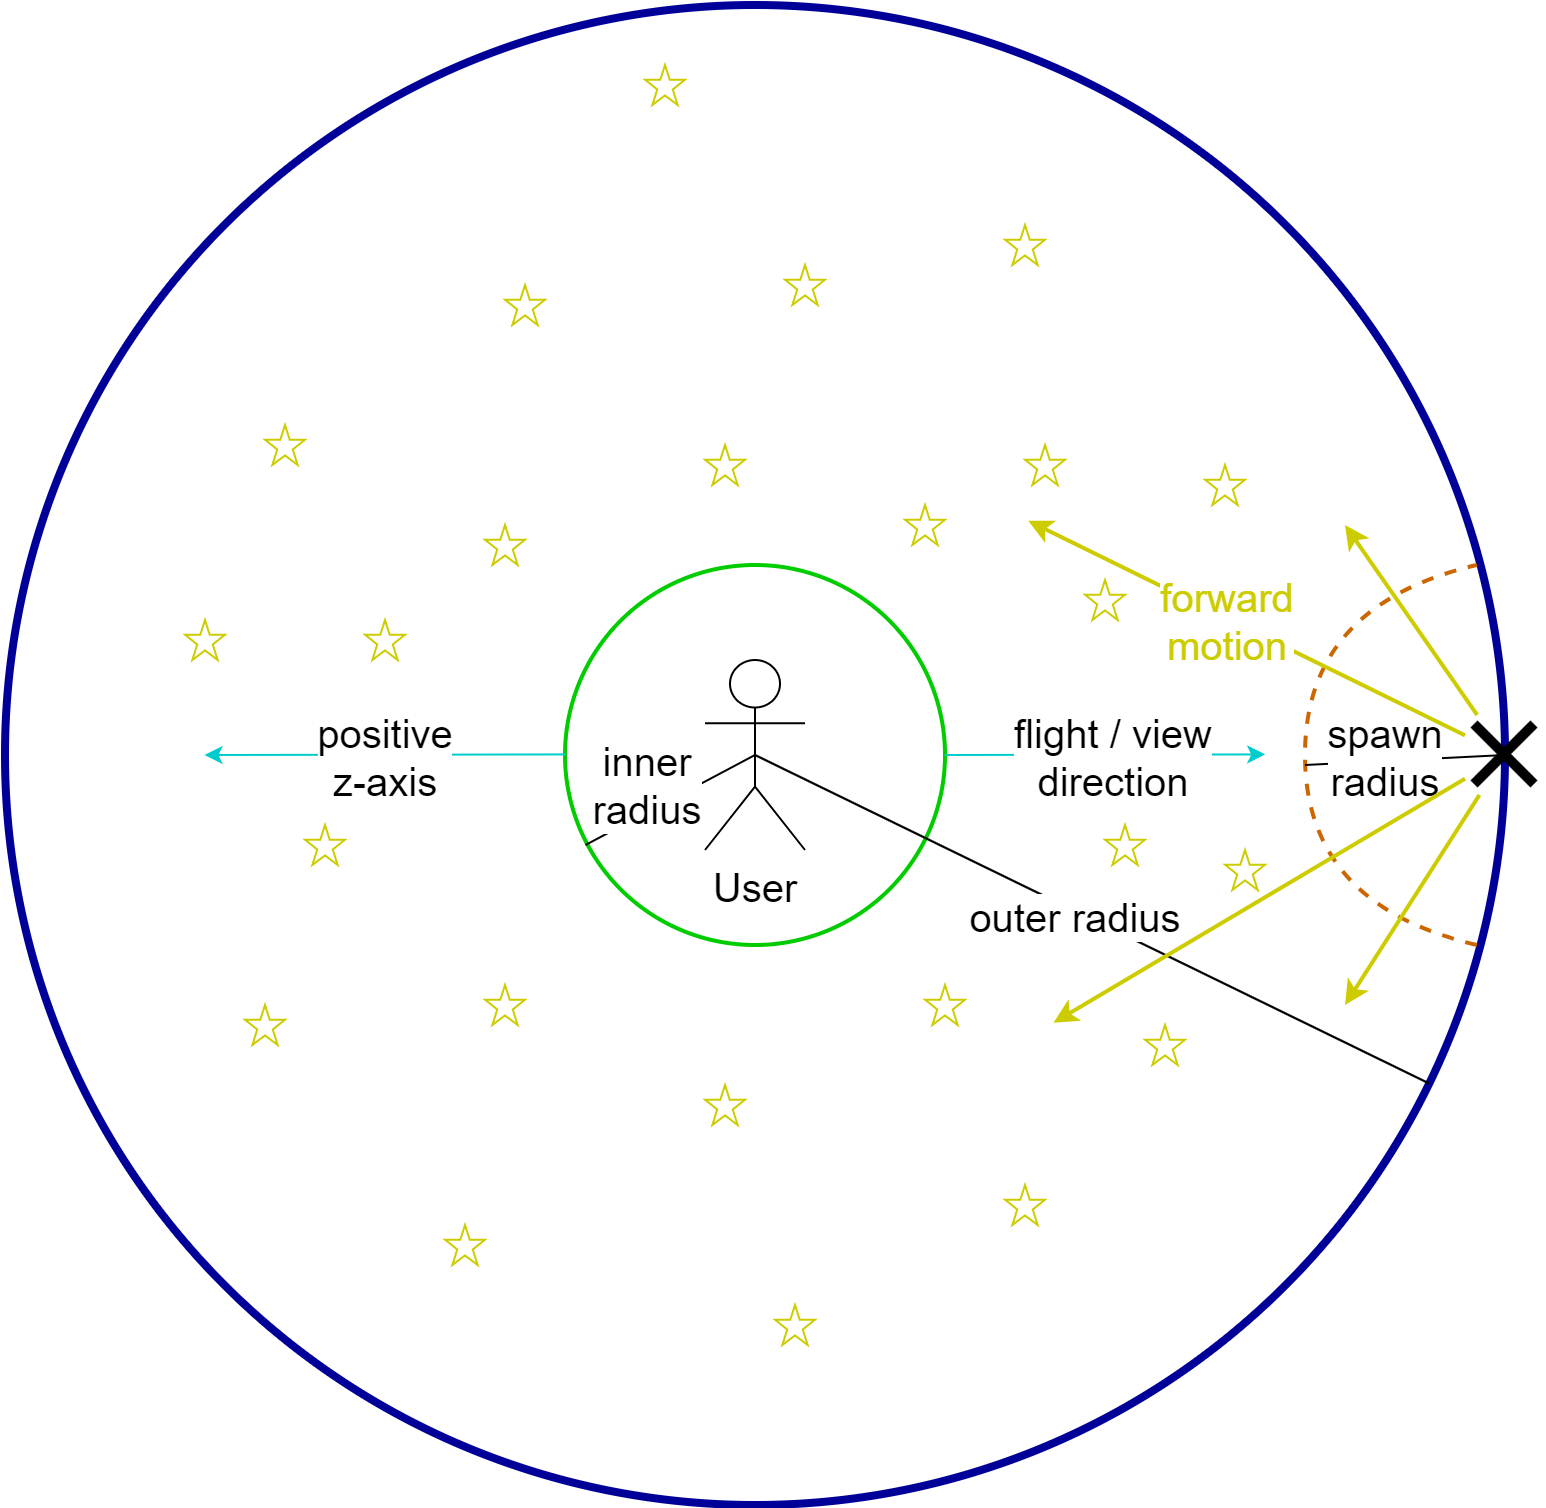
\includegraphics[width=.7\linewidth]{../pics/stars_sphere_schema}
	\caption{Schematic of the elements used in \lstinline|stars_sphere| to simulate space}
	\label{fig:space}
\end{figure}

A schematic of the spherical shell used to simulate space is shown in figure \ref{fig:space}. The outer radius determines the overall size of the sphere. A spherical region around the user that does not contain any stars is defined by the inner radius. This should include the complete bridge mesh to assure stars are only visible to the user on the view screen. Congruent with other parts of the plugin, the flight and view direction points along the negative $ z $-axis. 

Stars are rendered as small spheres whose radii follow a normal distribution. The shell is initialized with a constant number of stars with uniformally distributed positions. It saves the forward and angular speeds as float values. During a \lstinline|draw()| call, the method \lstinline|update()| calculates new positions for all stars. It can be summarized as follows:

\begin{algorithmic}
	\ForAll{stars}
		\State Move star away from origin
		\If{star is outside of shell}
			\State Respawn star
		\Else
			\State Rotate star around user
		\EndIf
	\EndFor
\end{algorithmic}

To somewhat simplify the math behind this calculation, I used the point on the outer hull right in front of the user as origin for the shell space, instead of the center of the shell. The origin is marked with a cross in figure \ref{fig:space}. A model view matrix then translates the shell to model space. 

When moving dead ahead (angular speeds are zero), stars are moved along the yellow "forward motion" arrows in figure \ref{fig:space}. The bigger the angle between their position vector and the positive $ z $-axis, the slower they move. More precisely, the length of a star's position vector is increased by the product of the cosine of the angle between the position vector and the positive $ z $-axis, and the general distance it covered, calculated from \lstinline|speed_ahead| and the time since the last update.

If a star moves outside the outer hull of the shell, its position is re-initialized randomly somewhere on a sphere of the spawn radius around the origin. It cannot be simply set to the origin because it needs a direction and the spawn radius should not be too small in order to also avoid the impression of stars spawning very densly.

An additional rotation is realized by simply rotating the stars around the user. After some experimenting, I realized the spawn sphere needs to be rotated inversely around the user as well to achieve a realistic experience and because otherwise, the newly spawned stars converge to a line at slow forward motion and fast rotations.

\section{Calibration} \label{sec:cal}
To make it possible to use \gls{VCP} in different rooms and setups, a calibration routine is required. This can be activated by joining index and thumb of one hand for three seconds. The objects in the scene are then no longer rendered.

The user position is determined from the \acrshort{hmd} if connected. Otherwise, the user is asked to tap index and thumb above their head and the position of the respective tracker at that time is used.

After that, a countdown of $ 3s $ is displayed and the user is instructed to hold their hands straight with the fingers pointing forward. At the end of the countdown, the hands are rendered again and the current pose is passed on to the \lstinline|hand| instances for calibration. It becomes a new reference pose from which all following orientations are inferred. 

This is necessary because the \Gls{AVR} does not give sufficiently accurate measurements for a period longer than a few minutes. Since the device apparently accumulates quaternions from instantaneous acceleration rates, the resulting rotations tend to quickly diverge from the actual hand pose. This effect is stronger if the device was moved even slightly during its intrinsic calibration at startup time.

Finally, the conn panel is moved close to the hands and the new $ z $-axis is set to run from the average of the hand positions and the user position. One can continue to adjust the panel position and $ z $-axis by moving their hands until satisfied. A final acknowledgement by tapping index and thumb ends the calibration.

Between two stages, a short feedback pulse  is generated by the actuators simultaneously to notify the user of the change. When the calibration is finished, a final pulse utilizes all actuators successively. The calibration can also be aborted resulting in three short pulses. One can then choose to reset to the previous calibration or keep the partially altered one.

\printglossary[type=gloss_terms]
\printglossary[type=gloss_acr]
\end{document}